\documentclass[aps, prc, 12pt, nofootinbib, showpacs, superscriptaddress, tightenlines, groupedaddress]{revtex4-2}
\usepackage{amsmath,amssymb,amsbsy,bm}
\usepackage{graphicx}
\usepackage{comment}
\usepackage{float}
\usepackage[colorlinks=true,linkcolor=blue,citecolor=blue,urlcolor=blue]{hyperref}
\usepackage[margin=0.75in]{geometry}
\usepackage{silence}
\WarningFilter{revtex4-2}{Repair the float}

%\usepackage[table]{xcolor}

\begin{document}

\title{Baryon Transport in Color Flux Tubes}
\author{Scott Pratt}
\affiliation{Department of Physics and Astronomy and National Superconducting Cyclotron Laboratory\\
Michigan State University, East Lansing, MI 48824~~USA}
\date{\today}

\pacs{}

\begin{abstract}
baryon transport ...
\end{abstract}

\maketitle

\section{Introduction}

\section{Baryon Transport from Merging Simple Flux Tubes}

Here, we consider the merging of two simple flux tubes into one. The term ``simple'' refers to the fact that the tube is generated by a single quark or anti-quark. In a simple tube, one can bisect the tube at any point and classify the color charge on each side of the bisection by its color multiplet, $p,q$. In SU(3), the multiplet is defined by two integers, which differs from SU(2), where a multiplet is denoted by a single number, $j$, e.g. the total angular momentum. Graphically, the state can be enumerated by the graphs in Fig. \ref{fig:pqmultiplet}. Multiplets denoted by $(p_1,q_1)$ and $(p_2,q_2)$ can be combined to create multiplets denoted by $(p',q')$. In SU(2), multiplets denoted by $j_1$ and $j_2$ only couple to singlet $j'=0$ if $j_1=j_2$. Similarly, for SU(3) two multiplets couple to a color singlet only if $p_1=q_2$ and $p_2=q_1$. For example, the $(1,0)$ multiplet (quark) and the $(0,1)$ multiplet (antiquark) can couple to a color singlet.

Before addressing merging, we review the case of a simple flux tube between a quark and antiquark. Figure \ref{fig:simpletube} illustrates how the flux can be reduced by quark-antiquark pairs tunneling out of the vacuum. 
\begin{figure}
\centerline{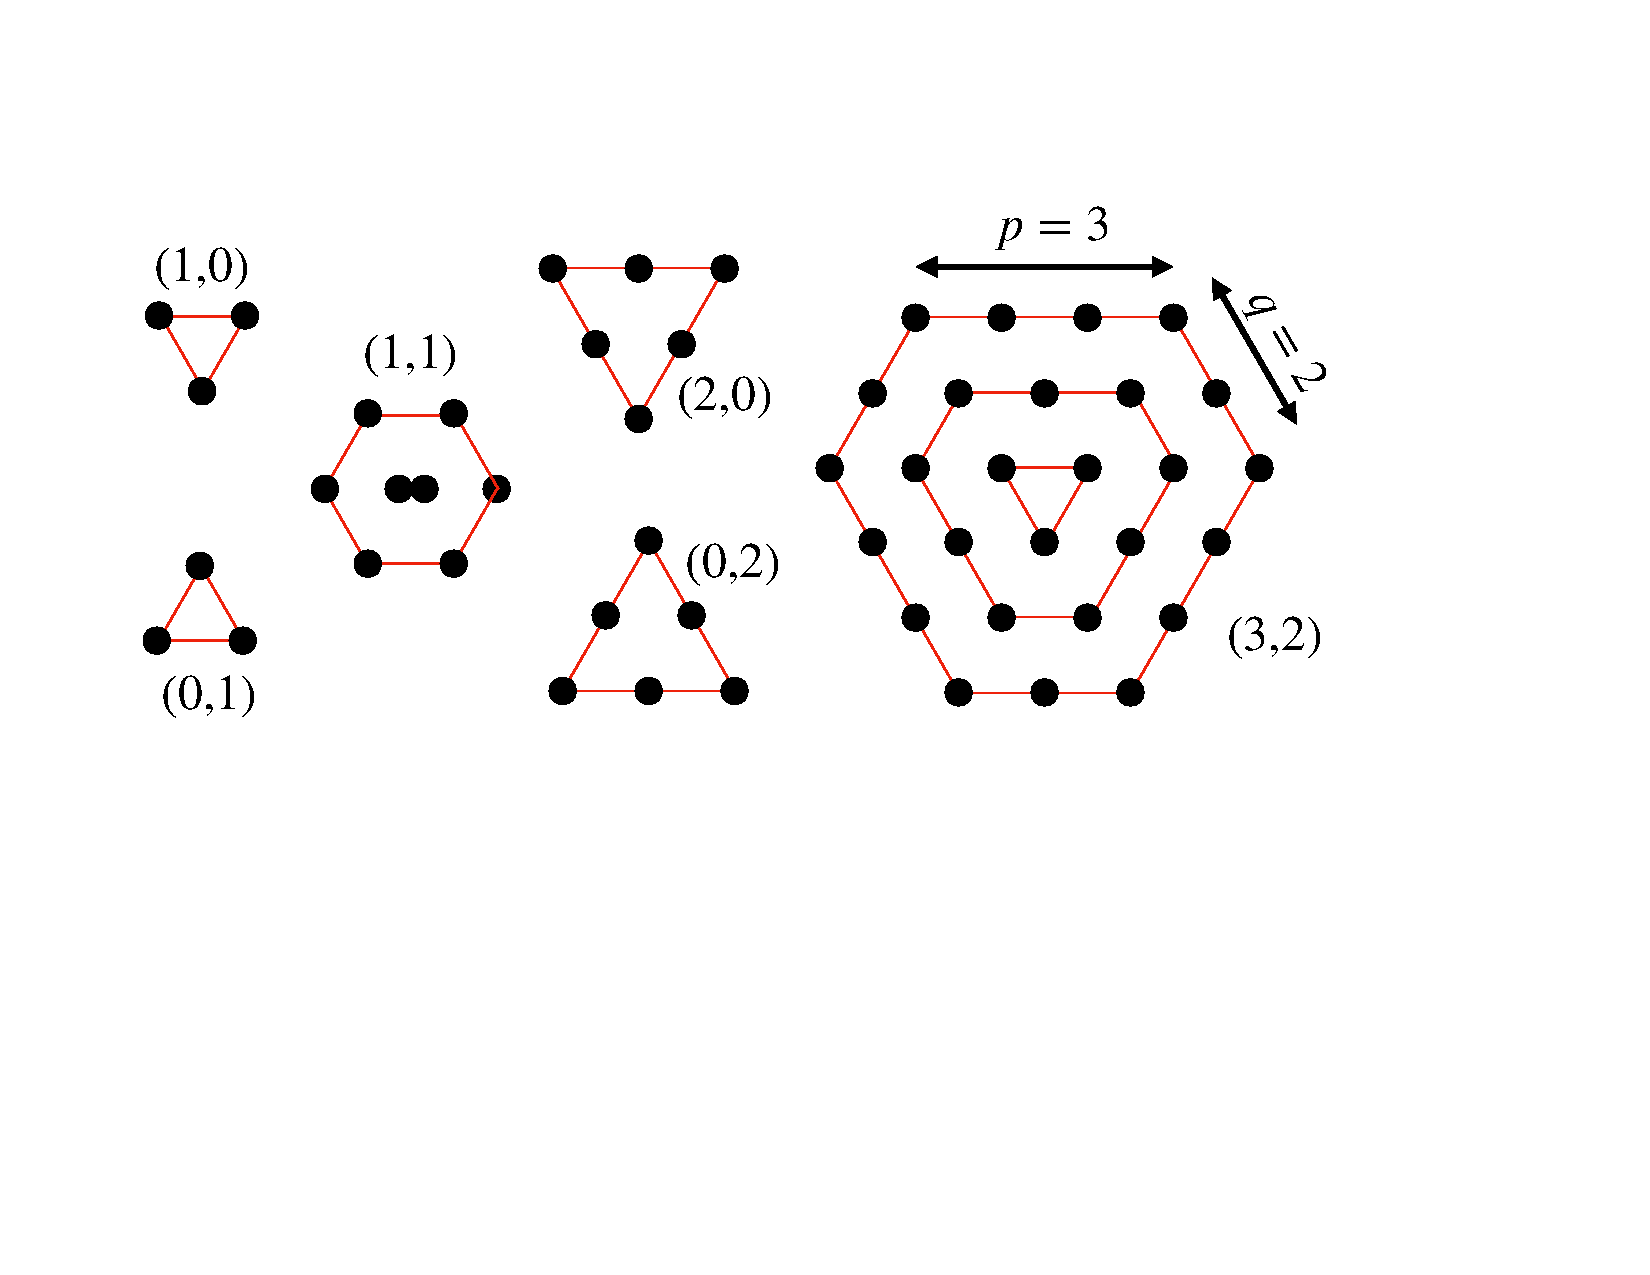
\includegraphics[width=0.6\textwidth]{figs/pqmultiplet.pdf}}
\caption{\label{fig:pqmultiplet}
Graphical representation of $(p,q)$ multiplets. The quark and antiquark color{} triplets are represented by $(1,0)$ and $(0,1)$, respectively, while the gluon octet is $(1,1)$. Each dot represents one projection of the multiplet, if the dot is on the outer ring. Subsequently, for the next inner-ring ring a dot represents two states, or three states for the next inner-ring, although the increasing degeneracy stops once a ring has either $p=0$ or $q=0$. The net degeneracy of the multiplet is $(p+1)(q+1)(p+q+2)/2$. In SU(2) one can combine multiplets of $j_1$ and $j_2$ to form several multiplets $j'$. Similarly, in SU(3) one can combine multiplets of $(p_1,q_1)$ and $(p_2,q_w)$ to form multiplets of several combinations of $(p',q')$.
}
\end{figure}

....

\begin{figure}
\centerline{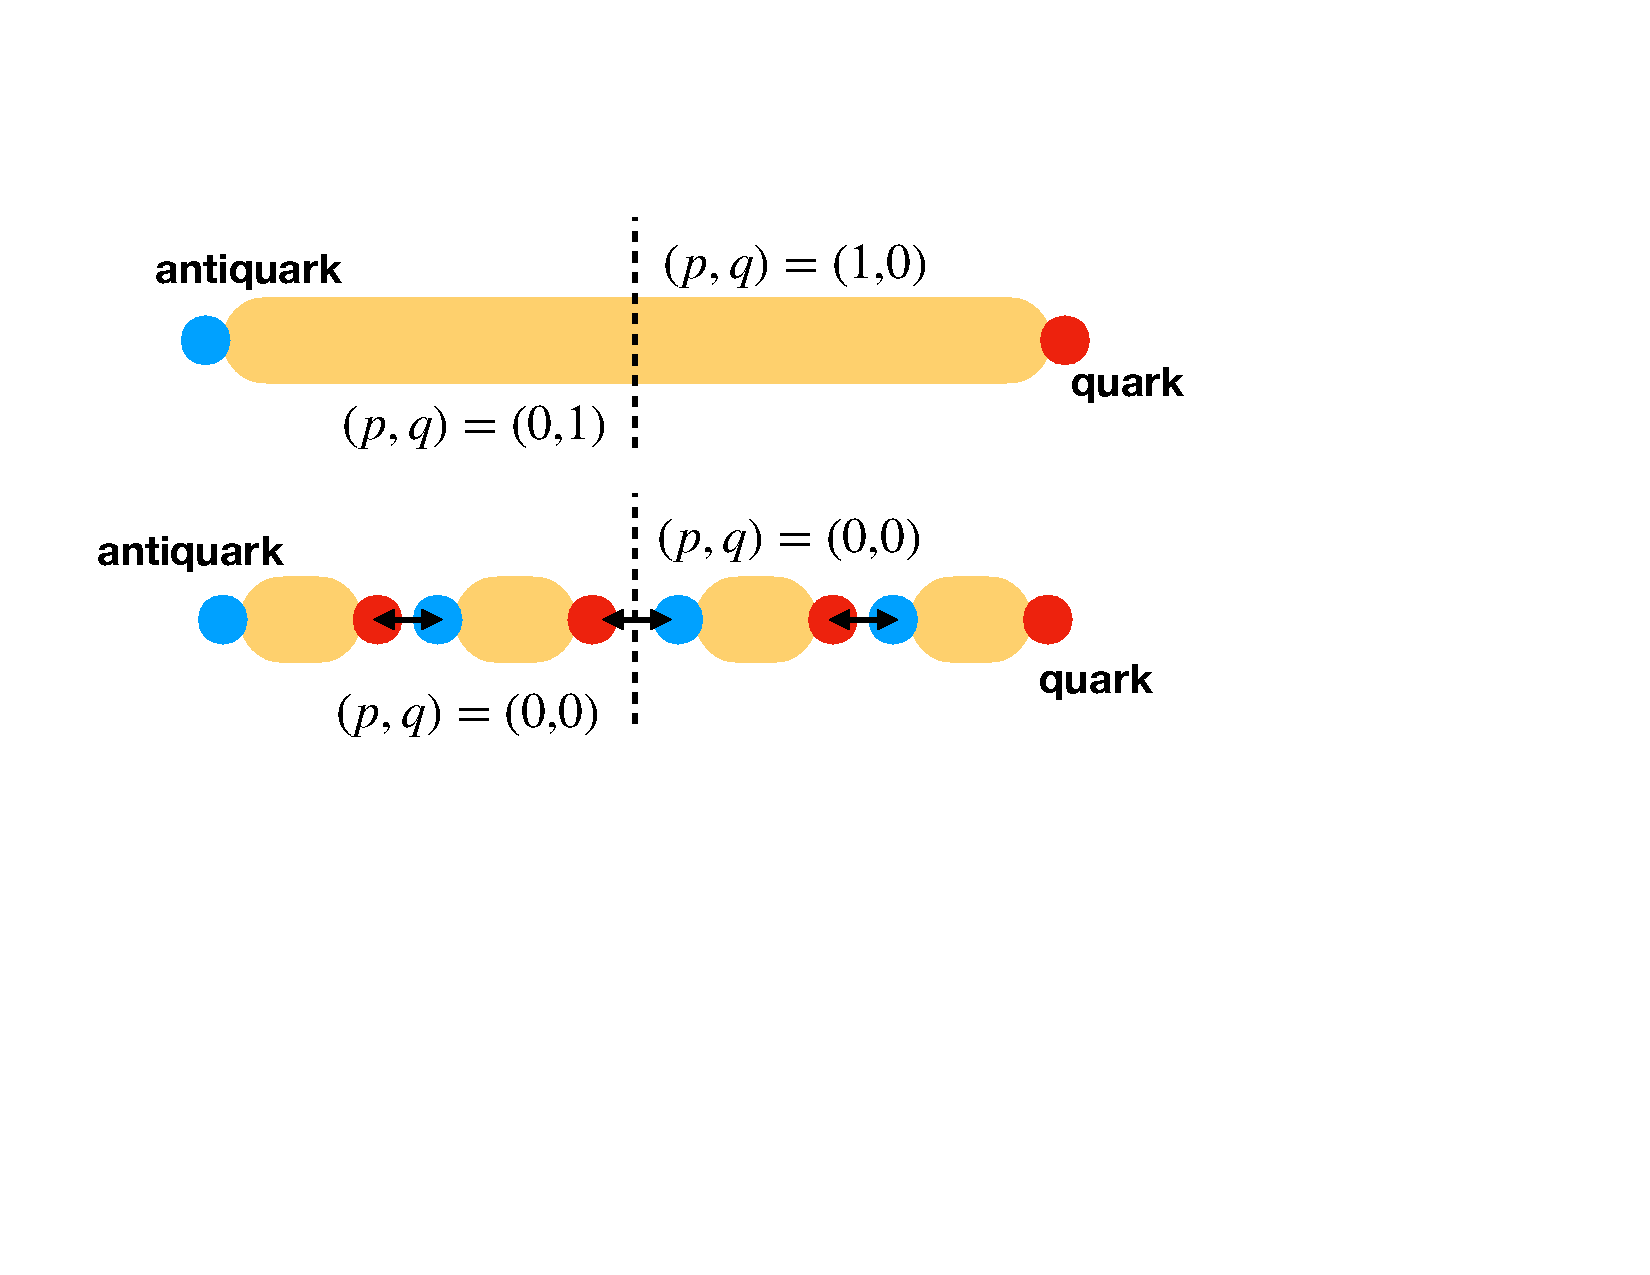
\includegraphics[width=0.4\textwidth]{figs/simpletube.pdf}}
\caption{\label{fig:simpletube}
A simple flux tube between a quark $(p=1,q=0)$ and an antiquark $(p=0,q=1)$ is illustrated in the upper panel, with the lighter and darker circles representing the quark and antiquark respectively. Drawing a vertical line through a flux tube divides space into two regions, the left side of the dashed line in a color multiplet $(p=1,q=0)$ and the right side in the multiplet $(p=0,q=1)$. The lower panel illustrates how quark-antiquark pairs can tunnel out of the vacuum so that the space between the tunneling quarks is free of color fields. Tunneling quark-antiquark pairs are denoted by the arrows.  Dividing space that does not bisect a tube results in both sides being in color singlets.
}
\end{figure}


\begin{figure}
\centerline{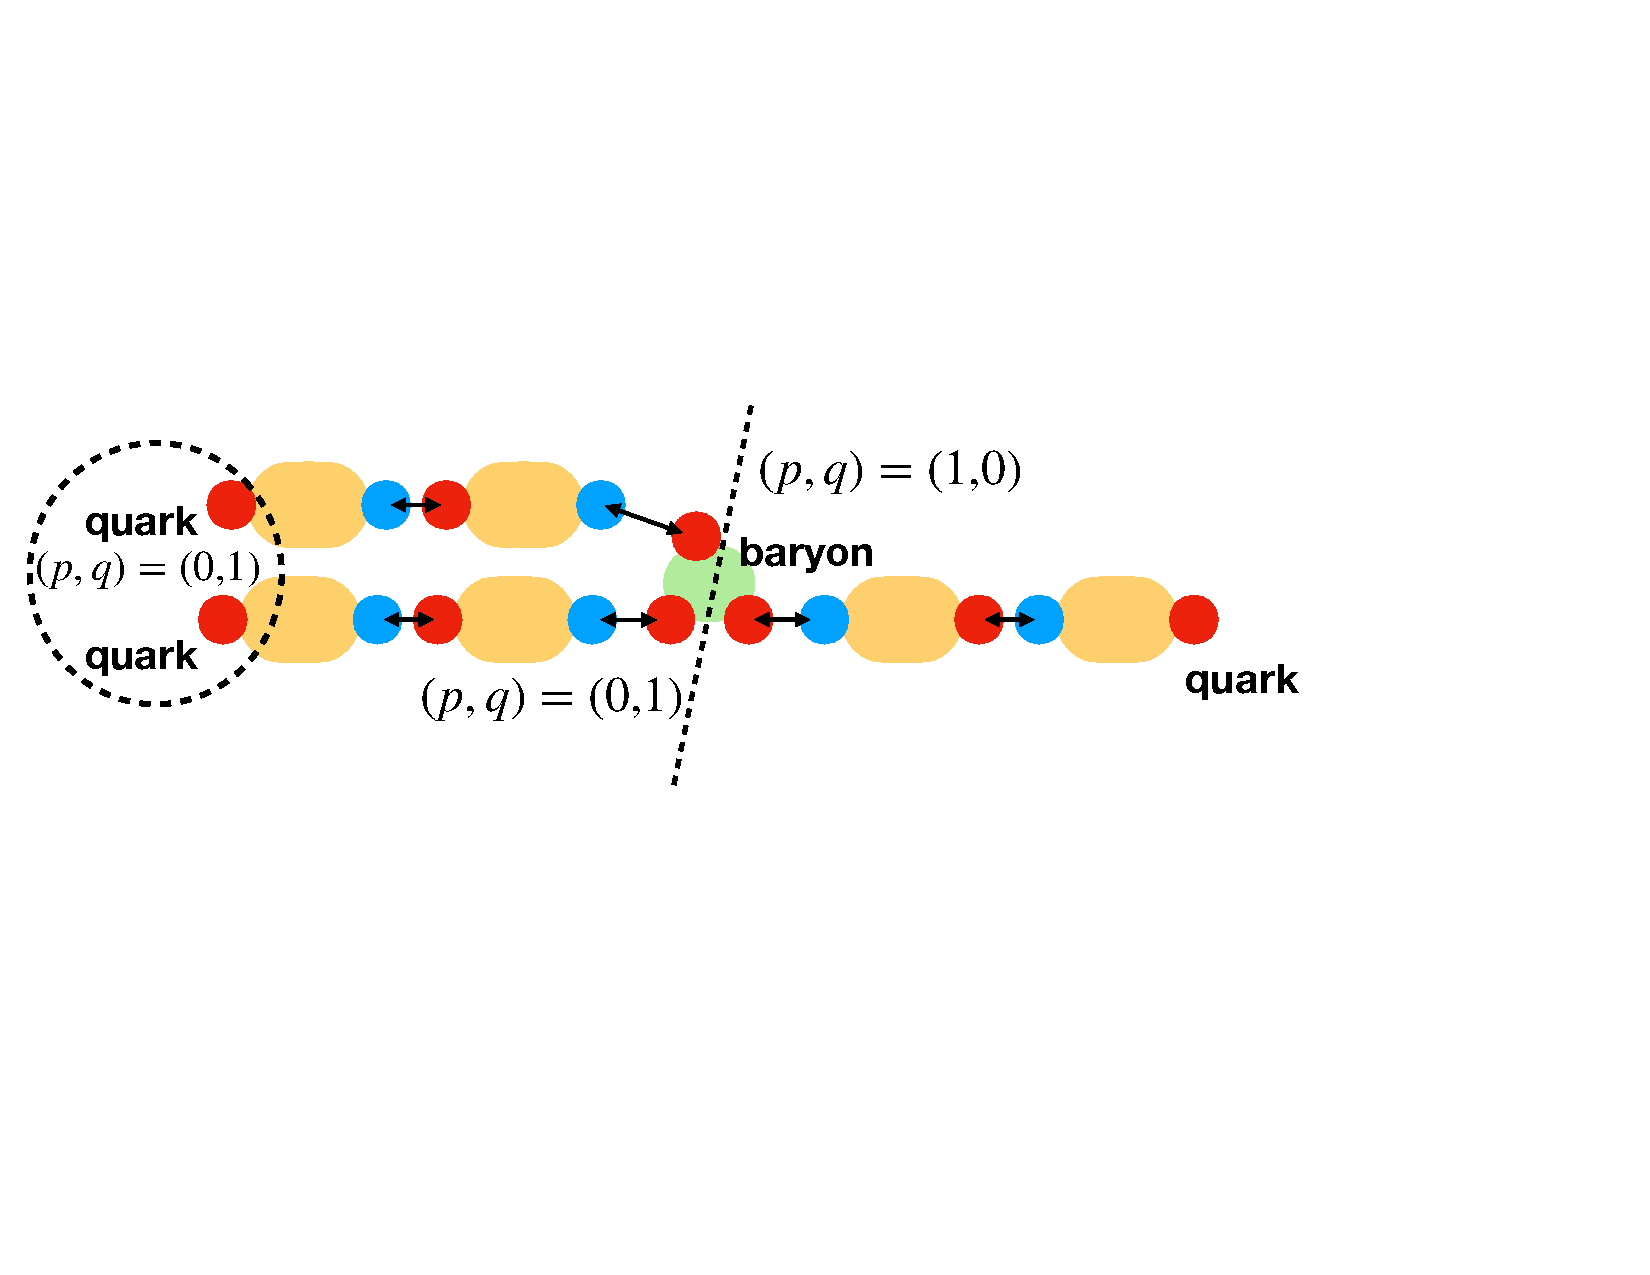
\includegraphics[width=0.48\textwidth]{figs/simplemerge.pdf}}
\centerline{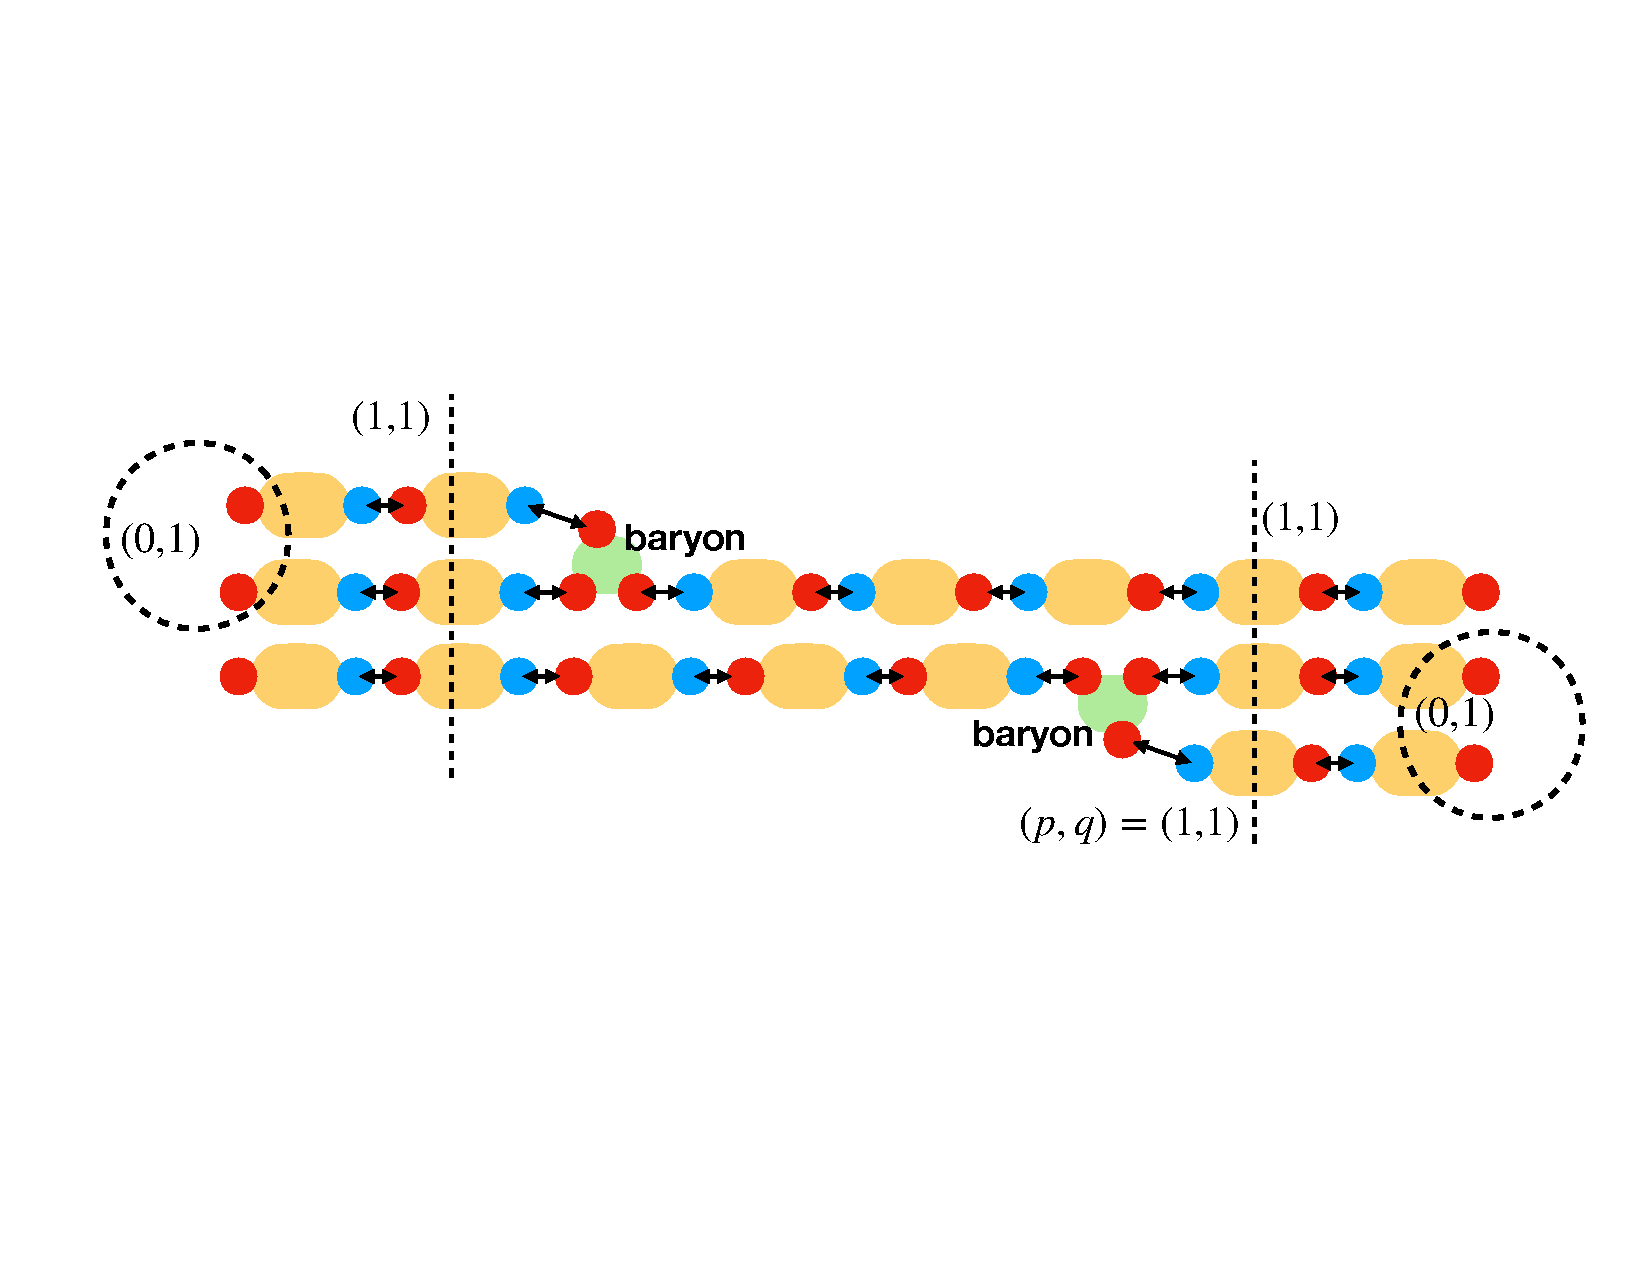
\includegraphics[width=0.6\textwidth]{figs/gluonexchange.pdf}}
\caption{\label{fig:merge}
Upper illustration: The merge of two tubes into one, where the left-hand side tubes begin with two quarks, and the right-hand side ends with one quark. The two quark multiplets couple to a $(0,1)$ multiplet, which then matches with the quark multiplet on the right. The baryon number, is then located at the point where the two tubes merged. This represents a situation where one quark is scattered far, from its original momentum, and the flux tubes must adjust to form local color singlets. The original quark pair must couple to $(p=0,q=1)$ if the overall configuration is to be a color singlet.\\
Lower illustration: This represents the case where two baryons exchange a soft gluon. In that case both of the baryons are transformed into $(p=1,q=1)$ multiplets. Assuming that for each baryon there is a diquark with $(p=0,q=1)$, the overall color singlet is restored by migrating the baryon number to the two places where the strings merge.\\
Darker circles represent quarks, while darker circles represent antiquarks. Ovals represent fluxtubes, and arrows describe quark-antiquark pairs that tunneled from vacuum.
}
\end{figure}


\section{Connecting Baryon Transport to Color Fields}

It is not obvious to see how baryon transport is connected to gluonic fields, $G^{\mu\nu}_a(x)$. Unlike the case for electric fields, gluon fields have a color index, $a$, and because all of nature is in a color singlet, the expectation of the field operators are zero, $\langle G^{\mu\nu}_a(x)\rangle=0$. Therefore, one must describe the fields through operators involving products of operators with color indices, i.e. corrrelators involving two or more operators with color indices. Further, gluons couple to color charge, not to baryon charge. The rather modest goal of this section is to write operators in terms of QCD field operators that represent the baryon polarization or baryon current and the the field-like operators that drive the polarization or current. These operators will be discussed in the context of flux tubes. None of the expressions derived here will be applied to quantitatively predict observables in this study. However, the presentation may help elucidate how fields in QCD can inspire baryon movement and separation.

\subsection{Color-Neutral Correlators}

Here, the color electric/magnetic field operators and the color current operators will be considered, $G^{\mu\nu}_a(x)$, and $j^\mu_a(x)$. Instead of the usual definition of such operators, we add an additional feature that enables the construction of gauge-invariant correlators. For any operator $\mathcal{O}(x)$, an additional attached operator is inferred \cite{Elze:1989un},
\begin{eqnarray}
\mathcal{O}_a(x)&\rightarrow \exp\{i\mathcal{P}\int d\vec{\ell}\cdot\vec{A}\}\mathcal{O}_a(x)\mathcal{P}\exp\{ig\int d\vec{\ell}\cdot\vec{A}\}.
\end{eqnarray}
Here, $\mathcal{P}$ is the path-ordering operator. With this definition, if some correlator $\langle\mathcal{O}_a(x)\mathcal{O}_a(x)\rangle$ is gauge invariant, then $\langle\mathcal{O}_a(x)\mathcal{O}_a(y)\rangle$ is also gauge invariant, though one needs to realize that the new correlator might depend on the actual path chosen. With this definition, one can write expressions that appear similar to those for Maxwell's equations,
\begin{eqnarray}
\partial_\mu j^\mu_a(x)&=&0,\\
\nonumber
\partial_\mu G^{\mu\nu}_a(x)&=&j^\nu_a(x).
\end{eqnarray}
Because all observables must be invariant to rotations in color space, one knows that $\langle\mathcal{O}_a\rangle=0$ and one must consider only colorless correlators. To find quantities which can be treated, at least to some degree, similarly as fields, we consider the following operators defined in terms of operators $j_a^\mu(x)$, where $a$ is a color index. 
\begin{eqnarray}
Q_{a,\Omega}&=&\int d\Omega_\mu j^{\mu}_a(x),\\
\nonumber
\langle Q^{(2)}_{\Omega_1,\Omega_2}\rangle&=&\int d\Omega_{1,\mu}d\Omega_{2,\nu}\langle j^\mu_a(x_1) j^\nu_a(x_2)\rangle,\\
\nonumber
&=&\langle Q_{a,\Omega_1}Q_{a,\Omega_2}\rangle,\\
\nonumber
\langle j^{(2)\nu}_{\Omega_1}(x)\rangle &=&\int d\Omega_{1,\mu} \langle j^\mu_a(x_1) j^\nu_a(x)\rangle\\
\nonumber
&=&\langle Q_{a,\Omega_1}j^\nu_a(x)\rangle.
\end{eqnarray}
Here, the superscripts $(2)$ reference the fact that these correlations are quadratic in the color charge. The volumes $\Omega_1$ and $\Omega_2$ can be any chosen volumes, and might be the same volume. If the volumes cover all space, and if the system is in an overall color singlet, $Q^{(2)}=0$. One can also define correlators using the fields,
\begin{eqnarray}
\langle G^{(2)\mu\nu}_{\Omega}(x)\rangle&=&\int d\Omega\langle Q_{a,\Omega}G^{\mu\nu}_a(x)\rangle.
\end{eqnarray}

As mentioned above, the correlators $\langle\mathcal{O}_a(x)\mathcal{P}_a(x)\rangle$ are gauge-invariant for any operators $\mathcal{O}$ or $\mathcal{P}$ that transform as the color charge, or equivalently as the 8 generators in SU(3). In fact, there are other combinations of operators that transform as color singlets. SU(3) has two Casimir operators, a Casimir being some combination of the group generators that commutes with the eight generators, $\lambda_a$. The first Casimir, often referred to as the quadratic Casimir
\begin{eqnarray}
C^{\rm(quadratic)}&=&\sum_a\lambda_a\lambda_a,
\end{eqnarray}
corresponds to the two-body correlators above. Unlike SU(2), SU(3) has a second Casimir, the cubic Casimir,
\begin{eqnarray}
C^{\rm(cubic)}&=&\sum_{abc}d_{abc}\lambda_a\lambda_b\lambda_c,
\end{eqnarray}
where $d_{abc}$ are the symmetric structure constants.
\begin{eqnarray}
\{\lambda_a,\lambda_b\}&=&\frac{4}{3}\delta_{ab}+d_{abc}\lambda_c.
\end{eqnarray}
It is this second Casimir that will be associated with baryon transport. Once can define a second set of current and charge-like operators, based on the cubic Casimir,
\begin{eqnarray}
\langle j^{(3)\mu}_{\Omega_1,\Omega_2}(x)\rangle &=&d_{abc}\langle Q_{a,\Omega_1}Q_{b,\Omega_1}j^\mu_c(x)\rangle,\\
\nonumber
\langle Q^{(3)}_{\Omega_1,\Omega_2,\Omega_3}\rangle&=&d_{abc}\int d\Omega_{1,\mu}d\Omega_{2,\nu}d\Omega_{3,\eta}\langle j^\mu_a(x_1) j^\nu_b(x_2)j^\eta_c(x_3)\rangle\\
\nonumber
&=&d_{abc}\langle Q_{a,\Omega_1}Q_{b,\Omega_2},Q_{c,\Omega_3}\rangle.
\end{eqnarray}
Again, the three volumes might or might not be the same. One can define the corresponding correlations involving field operators,
\begin{eqnarray}
\langle G^{(3)\mu\nu}_{\Omega_1,\Omega_2}(x)\rangle&=&d_{abc}\langle Q_{a,\Omega_1}Q_{b,\Omega_2}
G^{\mu\nu}_c(x)\rangle.
\end{eqnarray}

For the purposes of this discussion, two vector quantities are defined,
\begin{eqnarray}
E^{(2)}_{\Omega,i}(x)&=&\langle G^{(2)0i}_{\Omega}(x)\rangle,\\
\nonumber
E^{(3)}_{\Omega_1,\Omega_2,i}(x)&=&\langle G^{(3)0i}_{\Omega_1,\Omega_2}(x)\rangle.
\end{eqnarray}
These represent two measures of the color electric field, but are in fact correlators. They have no color index, as their color is defined relative to the color of the matter within the volume $\Omega$. These spatial vectors participate in two versions of Gauss's Law,
\begin{eqnarray}\label{eq:gauss}
 \oint d\vec{S}_2\cdot\vec{E}^{(2)}_{\Omega_1}(x_2)&=&Q^{(2)}_{\Omega_1,\Omega_2},\\
 \nonumber
 \oint d\vec{S}_3\cdot\vec{E}^{(3)}_{\Omega_1,\Omega_2}(x_3)&=&Q^{(3)}_{\Omega_1,\Omega_2,\Omega_3}.
\end{eqnarray}
Again, the volumes, $\Omega_1,\Omega_2,\Omega_3$, might or might not be chosen as being the same.

For a flux tube, where the fields are constant across a cross section $A$, one can define a volume $\Omega$ as all tube to the left of some position where we bisect the tube. If the charge with that volume are $Q^{(2)}_{\Omega,\Omega}$, Gauss's law states that the field is 
\begin{eqnarray}
E^{(2)}_{\Omega,\Omega}&=&\frac{1}{A}Q^{(2)}_{\Omega,\Omega}\\
\nonumber
&=&\langle Q_{a,\Omega}E_a\rangle.
\end{eqnarray}
For a single charge $a$, $\langle Q_{a,\Omega}Q_{a,\Omega}\rangle=\langle Q^{(2)}_{\Omega,\Omega}\rangle$. Thus, one can relate the energy density to the fields,
\begin{eqnarray}
 \epsilon&=&\frac{1}{2}\langle E_a^2\rangle\\
 \nonumber
 &=&\frac{1}{2}\frac{(E^{(2)}_{\Omega,\Omega})^2}{Q^{(2)}_{\Omega,\Omega}}.
\end{eqnarray}
The energy per unit length, or string tension is then
\begin{eqnarray}\label{eq:tension}
\frac{E}{L}&=&\frac{A}{2}\frac{(E^{(2)}_{\Omega,\Omega})^2}{Q^{(2)}_{\Omega,\Omega}}\\
\nonumber
&=&\frac{1}{2A}Q^{(2)}_{\Omega,\Omega}.
\end{eqnarray}
Thus, $Q^{(2)}$ is a measure of the energy per unit length of the tube, although if the area changes with the strength of the field, the correspondence is not purely linear.

At the end of this section it will be shown how $Q^{(3)}$ is related to baryon number. The meaning of the two charges are, roughly, that $Q^{(2)}$ describes the energy per unit length of the flux tube and $Q^{(3)}$ represents the propensity of the system to attract baryons vs. antibaryons.

\subsection{Kubo Relations for Conductivity and Polarizability}

Here, we consider a system divided into two volumes, $\Omega$ and a small adjacent volume $\delta\Omega$. We will consider the currents and polarizability in $\delta\Omega$, while using $\Omega$ to define the correlators. The field, $\vec{E}^{(3)}(\vec{r}\in\delta\Omega)$ and the current $\vec{j}^{(3)}(\vec{r}\in\delta\Omega)$ will be defined by the charge distribution in $\Omega$. First, to derive the Kubo relation for the conductivity, we consider the interaction with an color field,
\begin{eqnarray}
H^{\rm(int)}&=&-\int d^3r \rho_a(\vec{r})\vec{r}\cdot\vec{E}_a.
\end{eqnarray}
Following the usual steps for deriving the first-order perturbation correction to the current,
\begin{eqnarray}
\langle\vec{j}^{(3)}_{\Omega\Omega}(\vec{r})\rangle&=&-i\int d^3r'\int_{-\infty}^0 dt~\langle[\vec{j}^{(3)}(\vec{r}),
\int d^3r'~\rho_a(\vec{r}',t)\vec{r}'\cdot\vec{E}_a(\vec{r}',t)]\rangle\\
\nonumber
&=&id_{abc}\int d^3r'\int_{-\infty}^0 dt'~\langle[Q_{a,\Omega}Q_{b,\Omega}\vec{j}_c(\vec{r}),
\int d^3r'~\rho_d(\vec{r}',t')\vec{r}'\cdot\vec{E}_d(\vec{r}',t')]\rangle.
\end{eqnarray}
Here, $\vec{r}$ is inside $\delta\Omega$. Whereas the usual step in deriving Kubo relations is to treat the field as a constant external applied field, here the operator $\vec{E}_{\Omega,\Omega}^{(3)}(\vec{r}')$ is factored out instead. Only the $c=d$ term will contribute in this way.
\begin{eqnarray}
\langle\vec{j}^{(3)}_{\Omega\Omega}(\vec{r})\rangle&=&i\int_{-\infty}^0dt'~\int d^3r'\vec{r}'\cdot
\langle[\vec{j}_a(\vec{r}),\rho_a(\vec{r}',t')]\rangle  \vec{r}'\cdot\vec{E}^{(3)}_{\Omega,\Omega}({\rm in}~\delta\Omega).
\end{eqnarray}
Aside from the color indices, the prefactor to the electric field is the same as for calculating the Kubo relation for a normal electromagnetic field. This yields the result,
\begin{eqnarray}\label{eq:kubo}
\langle\vec{j}^{(3)}_{\Omega\Omega}(\vec{r})\rangle&=&\sigma \vec{E}^{(3)}_{\Omega,\Omega}(\vec{r}),\\
\nonumber
\sigma(\vec{r})&=&\frac{1}{2T}\int_{-\infty}^\infty dt'\int d^3r'~\langle\{\vec{j}_{ax}(\vec{r},t=0),\vec{j}_{ax}(\vec{r}',t')\}\rangle.
\end{eqnarray}
Thus, the conductivity, $\sigma$, doesn't include any mention of $\Omega$, and only depends on the local properties. It should be emphasized that Eq. (\ref{eq:jsigmaE}) one describes the contribution to the current due to the charge distribution in $\Omega$. If $\Omega$ is a subvolume, then other regions not only contribute, but their charges might interfere, either constructively or destructively, with those in $\Omega$.

If quarks and gluons are free, one can have currents and fields as presented above. However, if the world is comprised of color singlets, there is no current, but ther can be polarization. As will be discussed in the next subsection, the current $\vec{j}^{(3)}$ is correlated to a baryon current. Similarly, one can define a polarization of the color fields, that is also correlated to the polarization of baryon charge. Here, operators that play the role of polarization, and are also based on the cubic Casimir, are presented. 

The polarization operator is defined here as
\begin{eqnarray}
\vec{\mathcal{P}}_{\Omega_1,\Omega_2}^{(3)}(\vec{r})=\vec{r}d_{abc}\langle Q_{a,\Omega_1}Q_{b,\Omega_2}\rho_c(\vec{r})\rangle.
\end{eqnarray}
Using the same interaction as was used for the calculation of the conductivity above, one can calculate the thermal expectation of the polarization. Setting $\Omega_1=\Omega_2=\Omega$, and factoring out $E^{(3)}$ as was done earlier, one finds
\begin{eqnarray}\label{eq:polarization}
\langle\vec{\mathcal{P}}_{\Omega,\Omega}^{(3)}(\vec{r})\rangle&=&\kappa \langle\vec{E}^{(3)}_{\Omega,\Omega}(\vec{r})\rangle,\\
\nonumber
\kappa(\vec{r})&=&\frac{1}{3T}\int d^3r'\langle \rho_a(\vec{r})[\vec{r}\cdot\vec{r}']\rho_a(\vec{r}')\rangle.
\end{eqnarray}
As was the case for the conductivity, this expression for the polarizability does not depend on the the volume $\Omega$. If the charges appear in uncorrelated $\pm$ pairs, the polarizability becomes $g^2\langle(x_+-x_-)^2\rangle\rho_d$, where $\rho_d$ is the density of dipoles and $x_+-x_-$ is the distance between the two charges, $\pm g$. 



\subsection{Relation to Baryon Transport}

As was promised previoisl, the goal of this subsection is to demonstrate how baryon transport is related to the field $\vec{E}^{(3)}$, which was in turn related to the cubic Casimir. The quadratic and cubic Casimirs can be expressed in terms of the color multiplet labels $p$ and $q$ through
\begin{eqnarray}\label{eq:Q2Q3vspq}
C^{\rm quadratic}&=&(p^2+q^2+3p+3q+pq)/3,\\
C^{\rm cubic}&=&(p-q)(2p+q+3)(2q+p+3)/18.
\end{eqnarray}
The correlators $Q^{(2)}$ and $Q^{(2)}$ are given by the Casimirs,
\begin{eqnarray}
\langle p,q|Q^{(2)}_{\Omega,\Omega}|p,q\rangle&=&g^2C^{\rm quadratic},\\
\langle p,q|Q^{(3)}_{\Omega,\Omega,\Omega}|p,q\rangle&=&g^3C^{\rm cubic},\\
\end{eqnarray}
where $g$ is the couling constant, which plays the role of the fundamental charge, the equivalent of $e$ in electromagnetism. For a quark, $(p=1,q=0)$, one finds that $\langle Q^{(2)}\rangle=4/3$ and $\langle Q^{(3)}\rangle=(10/9)g^3$. An antiquark yields the opposite expectation,  $\langle Q^{(3)}\rangle=-(10/9)g^3$.

The multiplet labels $p$ and $q$ and the charge labels $Q^{(2)}$ and $Q^{(3)}$ represent alternative means to identify the multiplet. The labels $p$ and $q$ can be uniquely expressed in terms of the charges by solving a cubic equation. Defining
\begin{eqnarray}
c&\equiv&9\langle Q^{(2)}/g^2\rangle+9,\\
\nonumber
d&\equiv&18\langle Q^{(3)}/g^3\rangle,\\
\nonumber
\alpha&=&-2\pi /3+\frac{1}{3}\cos^{-1}[(3d/2c)\sqrt{3/c}],\\
\nonumber
y&=&2\sqrt{c/3}\cos\alpha,\\
\nonumber
x&=&-2+\sqrt{4+\langle Q^{(2)}/g^2\rangle-y^2/3},\\
\nonumber
p&=&(x+y)/2,\\
\nonumber
q&=&(x-y)/2.
\end{eqnarray}
The other two solutions to the cubic equation result in either $p$ or $q$ being negative. The solutions are unique in that no two combinations of  $Q^{(2)}$ and $Q^{(3)}$ result in the same $p$ and $q$.

Given that a quark has $p=1,q=0$ and an antiquark has $p=0,q=1$, it is natural to expect that a multiplet with $p>q$ will more likely dissolve into quarks, and that a multiplet with $q>p$ would more likely result in antiquarks. Given that $Q^{(3)}$ is an odd function of $p-q$ and that $Q^{(2)}$ is an even function, any correlation with baryon number is through the correlation with $Q^{(3)}$. Correspondingly, the field $E^{(2)}$ does not drive baryon transport, but $E^{(3)}$ does.

To express baryon transport, one must first understand $d\langle B\rangle/d\langle Q^{(3)}\rangle$. Once this is determined, the baryon current is
\begin{eqnarray}
\vec{j}_B(\vec{r})&=&\frac{d\langle B_{\delta\Omega}\rangle}{dQ^{(3)}_{\Omega,\Omega,\delta\Omega}}\sigma \vec{E}^{(3)}_{\Omega,\Omega}(\vec{r}).
\end{eqnarray}
Here, $\vec{r}\in\delta\Omega$. This represents the current inside the $\delta\Omega$ driven by the charge in $\Omega$. Statistical considerations give
\begin{eqnarray}
\frac{d\langle B_{\delta\Omega}\rangle}{dQ^{(3)}_{\Omega,\Omega,\delta\Omega}}&=&
\frac{\langle B_{\delta\Omega} Q^{(3)}_{\Omega,\Omega,\delta\Omega}\rangle}
{\langle [Q^{(3)}_{\Omega,\Omega,\delta\Omega}]^2  \rangle}.
\end{eqnarray}

One can follow the same arguments to calculate the baryon polarizability operator,
\begin{eqnarray}
\vec{P}_B(\vec{r})&=&\vec{r}d_{abc}\langle \rho_B(\vec{r})\rangle.
\end{eqnarray}
The ratio of $P_B$ to $P^{(3)}$ is the same as would be used for the current above. The baryon current and polarizability are then
\begin{eqnarray}
\langle\vec{j}_B(\vec{r})\rangle&=&\frac{d\langle B_{\delta\Omega}\rangle}{dQ^{(3)}_{\Omega,\Omega,\delta\Omega}}\sigma
\langle\vec{E}^{(3)}_{\Omega,\Omega}(\vec{r})\rangle,\\
\nonumber
\langle\vec{P}_B(\vec{r})\rangle&=&\frac{d\langle B_{\delta\Omega}\rangle}{dQ^{(3)}_{\Omega,\Omega,\delta\Omega}}\kappa
\langle\vec{E}^{(3)}_{\Omega,\Omega}(\vec{r})\rangle.
\end{eqnarray}

\subsection{Scaled Correlators}

The operators $Q^{(2)}, Q^{(3)},E^{(2)}(\vec{r})$ and $E^{(3)}(\vec{r})$ are correlators. If one assigns a dimension to charge coupling $g$, the units are $g^2$, $g^3$, $g^2/L^2$ and $g^3/L^3$, where $L$ refers to units of length. The operator $Q^{(2)}_{\Omega,\Omega}$ represents a fluctuation, and if one has a bulk system with independent color charges, and no long-range correlation, it would scale with the volume $\Omega$. If one were to consider $Q^{(3)}_{\Omega,\Omega,\delta\Omega}$ and the two field-like operators $E^{(2)}_{\Omega}(\vec{r})$ and $E^{(3)}_{\Omega,\Omega}(\vec{r})$, one would see that for independent charges, the fluctuations of these operators would scale, in the large $\Omega$ limit, as
\begin{eqnarray}
\langle [E^{(2)}_{\Omega}(\vec{r})]^2\rangle\propto \Omega,\\
\nonumber
\langle [Q^{(3)}_{\Omega,\Omega,\delta\Omega}]^2\rangle \propto \Omega^2\delta\Omega,\\
\nonumber
\langle [E^{(3)}_{\Omega,\Omega}(\vec{r})]^2\rangle\propto \Omega^2.
\end{eqnarray}
The correlator with baryon number would scale as
\begin{eqnarray}
\langle Q^{(3)}_{\Omega,\Omega,\delta\Omega}B_{\delta\Omega}\rangle\propto \Omega\delta\Omega.
\end{eqnarray}
Thus, if one were to consider a long flux tube, with $\Omega$ defined as everything to one side, the fluctuation of the field operators at the center of the tube would increase with the size of the tube,and the ratio of $d\langle B\rangle/d\langle Q^{(3)}\rangle$ would fall with size of the tube. 

One can scale the three operators above so that their dimensions and scaling with size are in line with the charge and field operators with which we are more accustomed.
\begin{eqnarray}
\tilde{\vec{E}}^{(2)}_{\Omega}(\vec{r})&\equiv&\frac{\tilde{\vec{E}}^{(2)}_{\Omega}(\vec{r})}{\langle Q^{(2)}_{\Omega,\Omega}\rangle^{1/2}},\\
\nonumber
\tilde{\rho}^{(3)}_{\Omega,\Omega}(\vec{r})&\equiv&\frac{\rho^{(3)}_{\Omega,\Omega}(\vec{r})}{\langle Q^{(2)}_{\Omega,\Omega}\rangle},\\
\nonumber
\vec{\tilde{\mathcal{P}}}_{\Omega,\Omega}^{(3)}(\vec{r})&\equiv&\frac{\vec{\tilde{\mathcal{P}}}_{\Omega_1,\Omega_2}^{(3)}}{\langle Q^{(2)}_{\Omega,\Omega}\rangle}\\
\nonumber
\tilde{Q}^{(3)}_{\Omega,\Omega,\delta\Omega}&\equiv&\frac{Q^{(3)}_{\Omega,\Omega,\delta\Omega}}{\langle Q^{(2)}_{\Omega,\Omega}\rangle},\\
\nonumber
\tilde{\vec{E}}^{(3)}_{\Omega,\Omega}(\vec{r})&\equiv&\frac{\vec{E}^{(3)}_{\Omega,\Omega}(\vec{r})}{\langle Q^{(2)}_{\Omega,\Omega}\rangle}.
\end{eqnarray}
With these definitions, $\tilde{Q}^{(3)}$ has dimensions of charge and $\tilde{E}^{(2)}$ and $\tilde{E}^{(3)}$ both have dimensions of charge per distance. The energy density is then more in line with $|\tilde{E}_{\Omega}^{(2)}(\vec{r})|^2/2$. Again, this would be, roughly, the energy density arising from the charges within $\Omega$. Correlators using any of the quantities scaled as above would then no longer grow with increasing $\Omega$ for systems with no long-range correlations. The charge correlators involving two operators labeled by $\delta\Omega$ would scale with $\delta\Omega$. 

Gauss's law relating  the scaled correlator $\tilde{E}^{(3)}$ to $\tilde{Q}^{(3)}$ is the same as that for the unscaled quantities.
\begin{eqnarray}
\oint_{\Omega} d\vec{A}\cdot\langle\vec{\tilde{E}}^{(3)}_{\Omega,\Omega}(\vec{r})\rangle&=&
\langle \tilde{Q}^{(3)}_{\Omega,\Omega,\Omega}\rangle,
\end{eqnarray}
or for arbitrary hyper-surfaces
\begin{eqnarray}\label{eq:gauss_scaled}
\oint_{\Omega} d\vec{A}\cdot\langle\vec{\tilde{E}}^{(3)}_{\Omega,\Omega}(\vec{r})\rangle&=&
\int d\Omega_{\mu}\cdot\langle \tilde{j}^{\mu(3)}_{\Omega,\Omega}(\vec{r})\rangle.
\end{eqnarray}

The Kubo relations for the scaled quantities become:
\begin{eqnarray}
\langle \vec{\tilde{j}}^{(3)}_{\Omega\Omega}(\vec{r})\rangle&=&\sigma \langle\tilde{\vec{E}}^{(3)}_{\Omega,\Omega}(\vec{r})\rangle,\\
\nonumber
\langle\tilde{\vec{\mathcal{P}}}_{\Omega,\Omega}^{(3)}(\vec{r})\rangle&=&\kappa \langle\tilde{\vec{E}}^{(3)}_{\Omega,\Omega}(\vec{r})\rangle.
\end{eqnarray}
The relations for baryon conductivity and polarizabilty become
\begin{eqnarray}\label{eq:kuboscaled}
\langle\vec{j}_B(\vec{r})\rangle&=&\frac{\langle B_{\delta\Omega}\tilde{Q}^{(3)}_{\Omega,\Omega,\delta\Omega}\rangle}
{\langle[\tilde{Q}^{(3)}_{\Omega,\Omega,\delta\Omega\rangle}]^2\rangle}
\sigma\langle\vec{\tilde{E}}^{(3)}_{\Omega,\Omega}(\vec{r})\rangle,\\
\nonumber
\langle\vec{P}_B(\vec{r})\rangle&=&\frac{\langle B_{\delta\Omega}\tilde{Q}^{(3)}_{\Omega,\Omega,\delta\Omega}\rangle}
{\langle[\tilde{Q}^{(3)}_{\Omega,\Omega,\delta\Omega\rangle}]^2\rangle}
\kappa\langle\vec{\tilde{E}}^{(3)}_{\Omega,\Omega}(\vec{r})\rangle.
\end{eqnarray}
The ratio of correlators in the Eq.s (\ref{eq:kuboscaled}) would then not grow with $\Omega$, approaching a constant. Thus, the fluctuation of the baryon current in the center of a long flux tube would be proportional to the fluctuation of $\tilde{E}^{(3)}$ which would not continue to grow with $\Omega$. 

\subsection{Applicability of Baryon Transport Relations}

The expressions in Eq. (\ref{eq:kuboscaled}) for the induced baryon current or polarizability provide insight into how color charge couples to baryon transport. For a system with non-zero conductivity, the application of the field $\vec{\tilde{E}^{{(3)}}}$ induces a current. Combined with Gauss's laws, Eq.s (\ref{eq:gauss}) and (\ref{eq:gauss_scaled}), one see how a sub-volume with quadratic charge $\tilde{Q}^{(2)}$ provides an energy per unit length to a tube of area $A$, in Eq. (\ref{eq:tension}). Further, if the sub-volume has a cubic charge, $\tilde{Q}$, it provides a field $E^{(3)}$, through Gauss's law. This field can then induce a baryon current, or if there is no conductivity, it induces a baryon polarization. 

These relations offer particularly nice insight into the flux tubes. In that case one first chooses some point along the tube, and the subvolume $\Omega$ is then chosed as every part of a flux tube to one side of the bisection point. By assuming that the field is constant across a cross-sectional area that bisects a tube, one knows both the field, and thus the induced baryon transport. However, because this insight was based on Gauss's law, it does not necessarily translate well outside the paradigm of a flux tube. Even for a spherical volume one can imagine that the system has zero quadratic or cubic charge. But, that charge might have a dipole, or quadrupole moment. Thus, in general, it is challenging to calculate the field correlators outside the flux tube approximation. Even in the flux tube approximation, the Kubo relations are questionable because they are based on perturbation theory due to a slowly-changing applied field. But in reality, such fields exist only in extremely dynamic systems, such as during the first half fm/$c$ of a hadronic collision. Even inside a hadron, the relations are difficult to motivate because the quarks and antiquarks are not isolated to one side of some volume. Finally, one should not forget that perturbation theory fails in QCD for any length or time scales $\gtrsim$ 1 fm.

Despite the limits to the applicability mentioned above, the relations do provide some useful insight, even if that insight mainly provide some theoretical backbone to heuristic arguments. In the next section, compound flux tubes, i.e. tubes where the sub-volumes are in states of higher-order color multiplets, are presented. This phenomenology might have more promise for further development, and perhaps provide predictive capability.

\section{Compound Flux Tubes}
\begin{figure}
\centerline{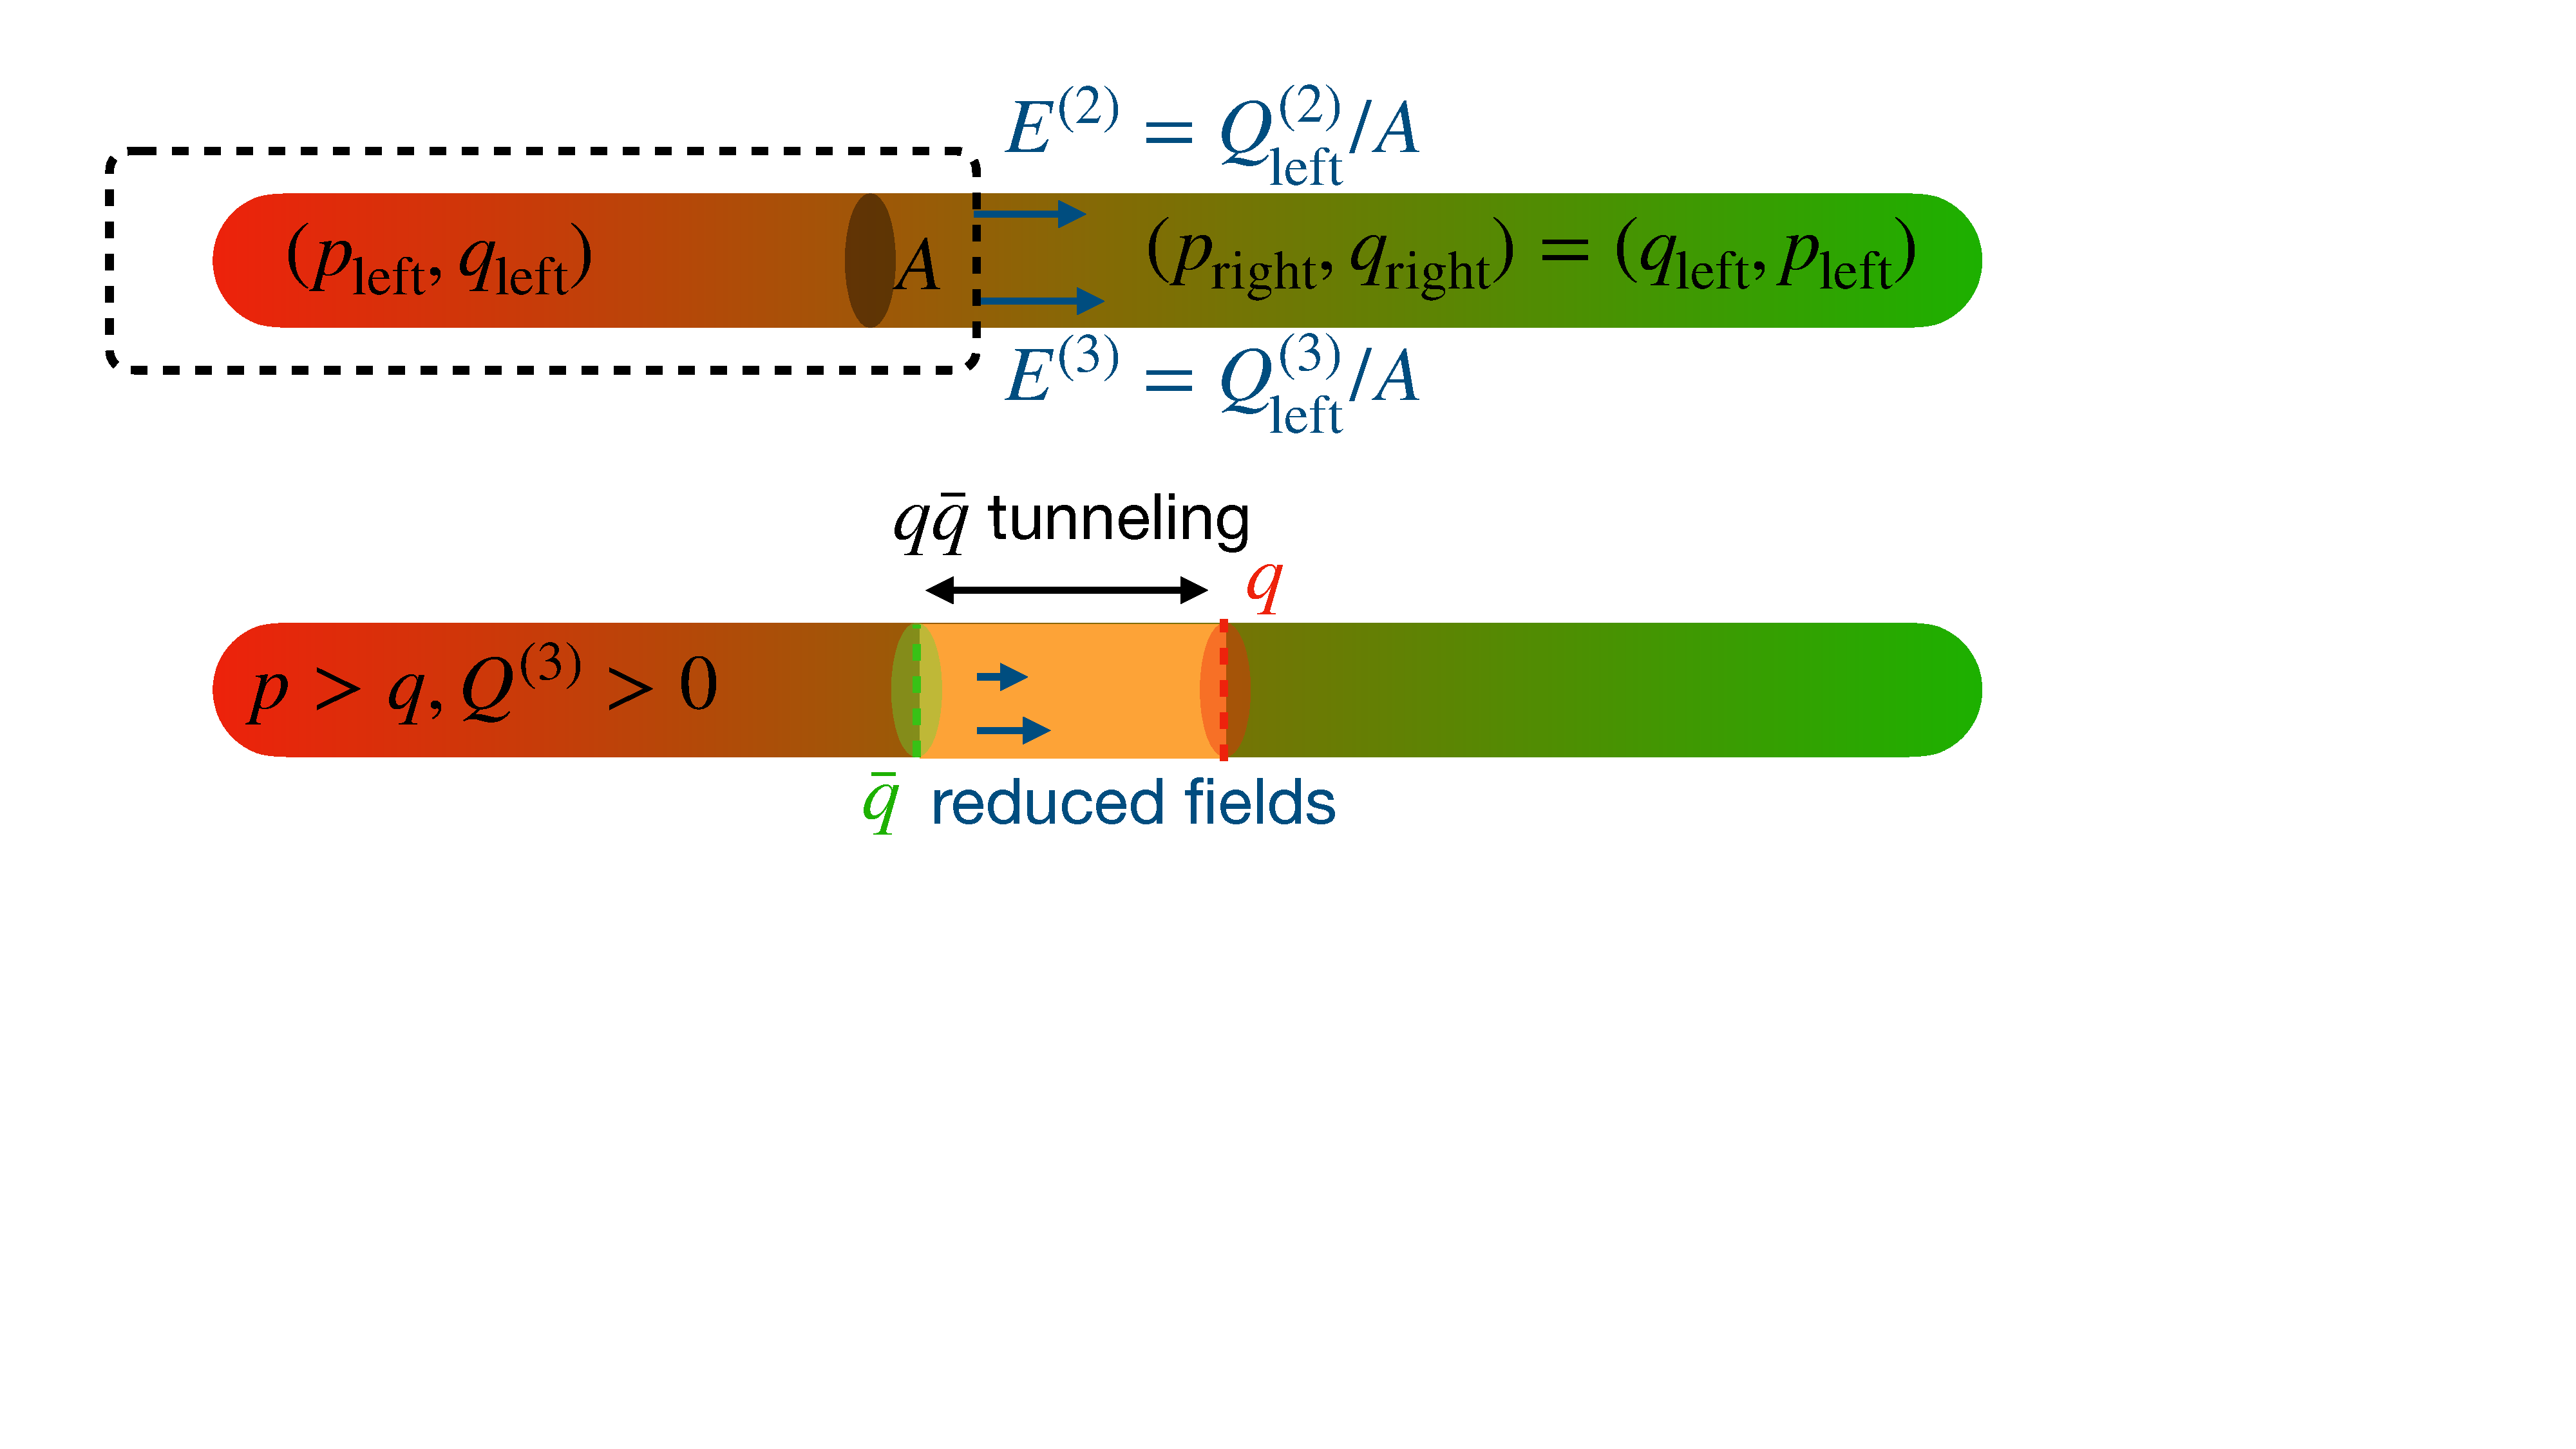
\includegraphics[width=0.5\textwidth]{figs/compoundtube.pdf}}
\caption{\label{fig:compoundtube}(color online)
The upper illustration show how a Gaussian surface isolates a flux tube into to parts. The color multiplets have interchanged values of $p$ and $q$. The energy density is defined by $\langle Q^{(2)}\rangle$, where the charge operators cover the left-hand side. 
}
\end{figure}

In Section \ref{sec:simpletubes}, simple flux tubes were discussed. The term ``simple'' was a tube with a quark at one end and an antiquark at the other. At any bisection point, the color multiplet to one side was either $(p=1,q=0)$ or $(p=0,q=1)$. Here, we discuss tubes where at the bisection point the multiplet to each might be described by a higher multiplet. For example havin a gluon to each side would be described by the octet $(p=1,q=1)$. By having multiple partons on a given side, any combination $(p,q)$ could be attained. The goal of this section is to investigate the possibilities of such combinations, and to understand how they might decay to the vacuum, which is a singlet $(p=0,q=0)$. The term ``compound'' tube refers to a tube with arbitrary $p$ and $q$. 

Figure \ref{fig:compoundtube} illustrates a flux tube , where a Gaussian surface bisects the tube at some point as shown in the upper diagram. If the multiplet to one side is $(p,q)$ the multiplet describing the opposite side is $(q,p)$. Otherwise, the tube would not be in an overall color singlet. At the point of the bisection, the field-like color correlators are given by the color charges $Q^{(2)}$ and $Q^{(3)}$, which are simple functions of $p$ and $q$ defined in Eq. (\ref{eq:Q2Q3vspq}). The field energy is determined by $\langle Q^{(2)}\rangle_{\rm left}$ and the propensity to induce a baryon current is described by $\langle Q^{(3)}\rangle_{\rm left}$. If a $q\bar{q}$ pair tunnels through the vacuum, as shown in the lower diagram of Fig. \ref{fig:compoundtube}, the color multiplet of matter to the left of a point between the $q\bar{q}$ pair changes, and if it lowers $\langle Q^{(2)}\rangle_{\rm left}$, the energy density of the region between the $q\bar{q}$ is reduced. Eventually, $q\bar{q}$ pairs must be produced in such a way that one reaches a color singlet with $\langle Q^{(2)}\rangle_{\rm left}$.

For the field-like correlators at some point to vanish, partons must pass the point where the defining Gaussian surface intersects the flux tube. When a parton pass through the surface, the color state of the matter changes. If the initial multiplet is $(p_i,q_i)$ the available final states $(p_f,q_f)$ depend on whether the parton was a gluon, a quark or an antiquark.
\begin{eqnarray}
(p_i,q_i)+{\rm gluon}&\rightarrow& (p_f,q_f)=\left\{
\begin{array}{l}
(p_i+2,q_i-1)\\
(p_i+1,q_i-2)\\
(p_i-1,q_i+2)\\
(p_i-2,q_i+1)\\
(p_i+1,q_i+1)\\
(p_i-1,q_i-1)\\
(p_i,q_i)~~({\rm two~multiplets})
\end{array}
\right.\\
\nonumber
(p_i,q_i)+{\rm quark}&\rightarrow& (p_f,q_f)=\left\{
\begin{array}{l}
(p_i+1,q_i)\\
(p_i,q_i-1)\\
(p_i-1,q_i+1)
\end{array}
\right.\\
\nonumber
(p_i,q_i)+{\rm antiquark}&\rightarrow& (p_f,q_f)=\left\{\begin{array}{l}
(p_i,q_i+1)\\
(p_i-1,q_i)\\
(p_i+1,q_i-1)
\end{array}
\right.
\end{eqnarray}

If the initial tube is created by exchanging only gluons across the bisection point, the available multiplets must have $p-q$ in multiples of three. Even though such states were created by gluons passing through, both $p-q$ and $\langle Q^{(3)}\rangle_{\rm left}$ can be non-zero. Thus, they can induce baryon transport across the bisection point. However, if the decay involves gluon pairs, one can also return to the ground state without any quarks passing the bisection. If quarks and or antiquarks were initially exchanged across the bisection, one can also return to the ground state through the creation of gluon pairs if the difference in the quark number is a multiple of three. One can define a quark excess number as
\begin{eqnarray}
B_x&=\left\{\begin{array}{rl}
1,&N_{\rm quarks}-N_{\rm antiquarks}=\cdots,-5,-2,1,4,7\cdots\\
-1,&N_{\rm quarks}-N_{\rm antiquarks}=\cdots,-7,-4,-1,2,5\cdots\\
0, &N_{\rm quarks}-N_{\rm antiquarks}=\cdots,-6,-3,0,3,6\cdots
\end{array}\right.
\end{eqnarray}








\begin{figure}
\centerline{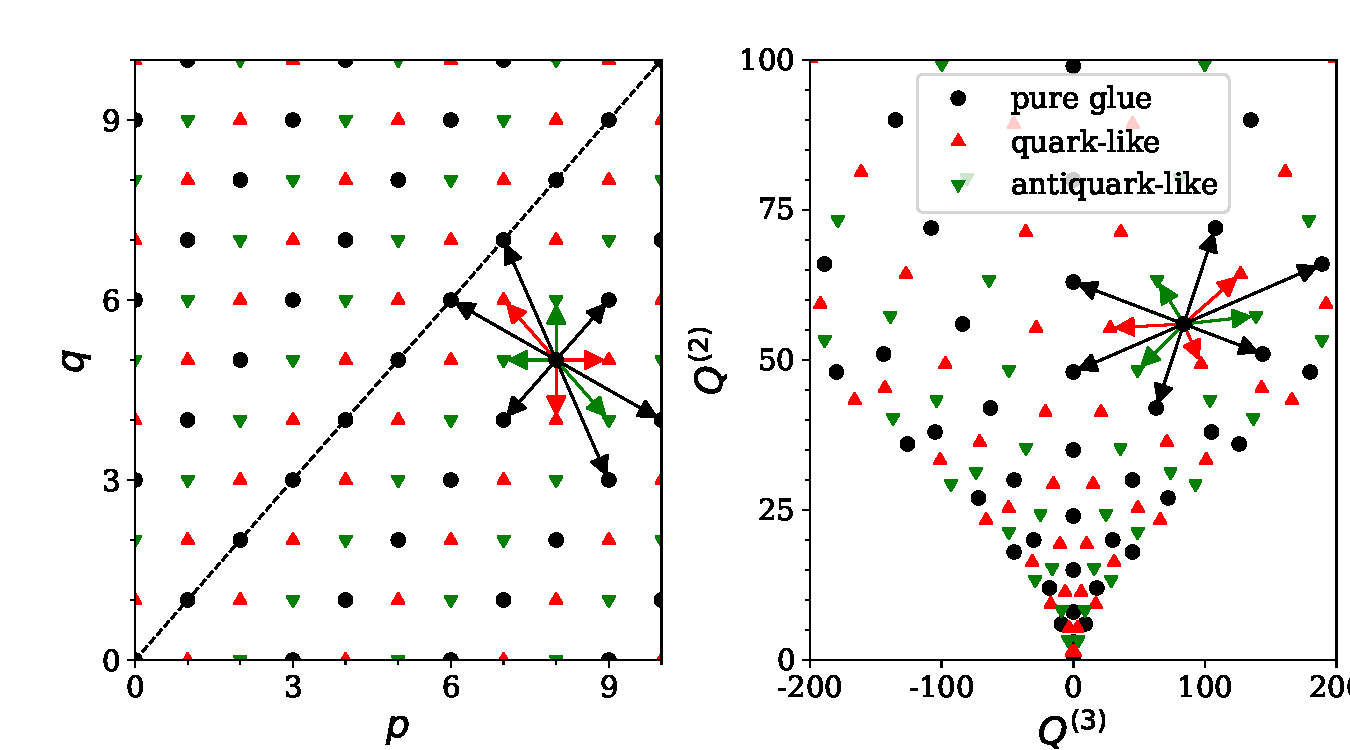
\includegraphics[width=0.75\textwidth]{figs/pq3.pdf}}
\caption{\label{fig:pq3}(color online)
Color multiplets are shown as a function of $(p,q)$ in the left-side panel. Starting from the singlet, ($p=0,q=0$), one can combine gluons to reach any of the multiplets denoted by black circles. These ``gluon-like'' states,  can also be reached by combining quarks and antiquarks if the difference of the number of quarks and antiquarks is a multiple of three. To reach a ``quark-like state'', one where $(p-q)/3$ has a remainder of +1 or -2, one can add a quark to a gluon-like state. One can reach an ``antiquark-like state'', one where the remainder of $(p-q)/3$ is -1 or 2, by adding an antiquark to a gluon-like state. The heavy black lines show the states available after adding either a gluon (heavy black line), an antiquark (light green line) or a quark (light dotted line). If gluon creation is possible, the most efficient way the system can reach a color singlet is to create gluon pairs, or perhaps one quark or antiquark depending on whether the original state is gluon-like, quark-like or antiquark-like. If gluonic steps are not permitted the most efficient decay mechanism is to add $p$ antiquarks and $q$ quarks. The right-side panel represents the same states, but the states are plotted as $\langle Q^{(2)}\rangle$ vs $\langle Q^{(3)}\rangle$. In this basis the energy per unit length is a function of $\langle Q^{(2)}\rangle$ and the field driving the baryon current is $\langle Q^{(3)}\rangle$.}
\end{figure}




\begin{acknowledgments}
This work was supported by the Department of Energy Office of Science through grant number DE-FG02-03ER41259.
\end{acknowledgments}

\bibliography{btransport}

\end{document}
